\chapter{Metode Penelitian}
Pada bab ini, akan dilakukan penjelasan mengenai alat dan bahan pendukung dari tugas akhir ini.
Alat dan bahan tersebut berupa perangkat keras, perangkat lunak, dan bahan data.
Selain itu, bab ini juga akan memaparkan mengenai alur dan urutan pengerjaan Tugas Akhir.
\section{Alat dan Bahan Tugas akhir}
Alat yang digunakan untuk mengembangkan Aplikasi ini terdiri dari Perangkat Keras dan Perangkat Lunak.
\subsection{Alat Tugas akhir}
\subsubsection{Perangkat Keras}
\begin{enumerate}
	\item \textit{laptop} dengan spesifikasi minimum anu, 
	pada tugas akhir ini digunakan \textit{Laptop Asus ROG Zephyrus G14} dengan spesifikasi sistem operasi Windows 11, \textit{processor} AMD Ryzen 5 4600HS with Radeon Graphics @ 3,00 GHz, memori 16GB DDR4, grafis NVIDIA GeForce GTX 1650Ti (4GB), SSD 512GB.
	\item \textit{Smartphone} dengan spesifikasi minimum anu, pada tugas akhir ini digunakan \textit{Smartphone Samsung Galaxy S20 Ultra} dengan spesifikasi OS Android 13 (Tiramisu), CPU Octa-core (2x2.73 GHz Mongoose M5, 2x2.50 GHz Cortex-A76, 4x2.0 GHz Cortex-A55), GPU Mali-G77 MP11, Internal 128 GB, 12GB RAM.
\end{enumerate}

\subsubsection{Perangkat Lunak}
\begin{enumerate}
	\item \textit{laptop} dengan spesifikasi minimum anu, 
	pada tugas akhir ini digunakan \textit{Laptop Asus ROG Zephyrus G14} dengan spesifikasi sistem operasi Windows 11, \textit{processor} AMD Ryzen 5 4600HS with Radeon Graphics @ 3,00 GHz, memori 16GB DDR4, grafis NVIDIA GeForce GTX 1650Ti (4GB), SSD 512GB.
	\item \textit{Smartphone} dengan spesifikasi minimum anu, pada tugas akhir ini digunakan \textit{Smartphone Samsung Galaxy S20 Ultra} dengan spesifikasi OS Android 13 (Tiramisu), CPU Octa-core (2x2.73 GHz Mongoose M5, 2x2.50 GHz Cortex-A76, 4x2.0 GHz Cortex-A55), GPU Mali-G77 MP11, Internal 128 GB, 12GB RAM.
\end{enumerate}
% \begin{enumerate}
% 	\item Microsoft Visual Studio Code 2022
% 	\item Figma
% \end{enumerate}
\newpage
\subsection{Bahan Tugas akhir}
Bahan yang digunakan untuk Tugas Akhir ini ialah sebagi berikut :
\begin{enumerate}
	\item Materi mata kuliah \textit{System Diagnosis Berbasis Pembantu Keputusan} (SBPK) dari Departemen Teknik Elektro dan Teknologi Informasi berupa file .pptx
	\item Data hasil wawancara pada Mahasiswa Teknik Biomedis yang telah memperolah mata kuliah SDBPK untuk kebutuhan \textit{User Persona}
\end{enumerate}
% \begin{itemize}
% 	\item Dataset pihak lain yang diperoleh dengan izin atau dalam lisensi yang diizinkan untuk digunakan secara langsung 
% 	\item Dataset pihak pertama yang disusun sendiri melalui quisioner, observasi, atau interview 
% 	\item Dokumen panduan yang mengacu pada standar, hasil tugas akhir, atau artikel yang disitasi dan digunakan.
% \end{itemize}


\section{Metode yang Digunakan}

Metode yang akan dipakai dalam tugas akhir akan dibagi menjadi Pengembangan Aplikasi, Pengembangan Desain Aplikasi, serta Pengujian Aplikasi dan Efektifitas Aplikasi.
Untuk pengembangan Aplikasi pada Tugas Akhir ini akan diterapkan metode FDD atau \textit{Feature-Driven Development}, metode ini digunakan karena

Untuk Pengembangan Design Gamifikasi pada tugas akhir ini akan diterapkan metode pengembangan.....

Untuk pengujiannya sendiri, aplikasi ini akan diuji dengan Black Box testing untuk menguji Fitur fitur.....



\section{Alur Tugas Akhir}

Tugas Akhir ini akan dibagi menjadi tahap \textit{Development} dan Tahap pengujian.
Untuk tahap \textit{Development} sendiri akan menggunakan metode \textit{Feature-Driven Development} untuk mengembangkan Softwarenya.
Proses \textit{Development} ini termasuk juga proses perancangan Gamifikasi yang akan diadopsi pada Aplikasi.
Untuk tahap pegujian, penulis akan mengujikan Fungsionalitas Aplikasi yang telah dikembangkan menggunakan Pengujian \textit{Black Box Testing}.
Kemudian dilanjutkan dengan Pengujian \textit{System Usability Scale} dan \textit{User Experience Questionnaire} untuk mengevaluasi pengalamaan pengguna mengenai Aplikasi yang telah dikembangkan.
Secara keseluruhan, Alur Tugas Akhir ini dapat dilihat pada gambar ....
\begin{figure}[H]
	\centering
	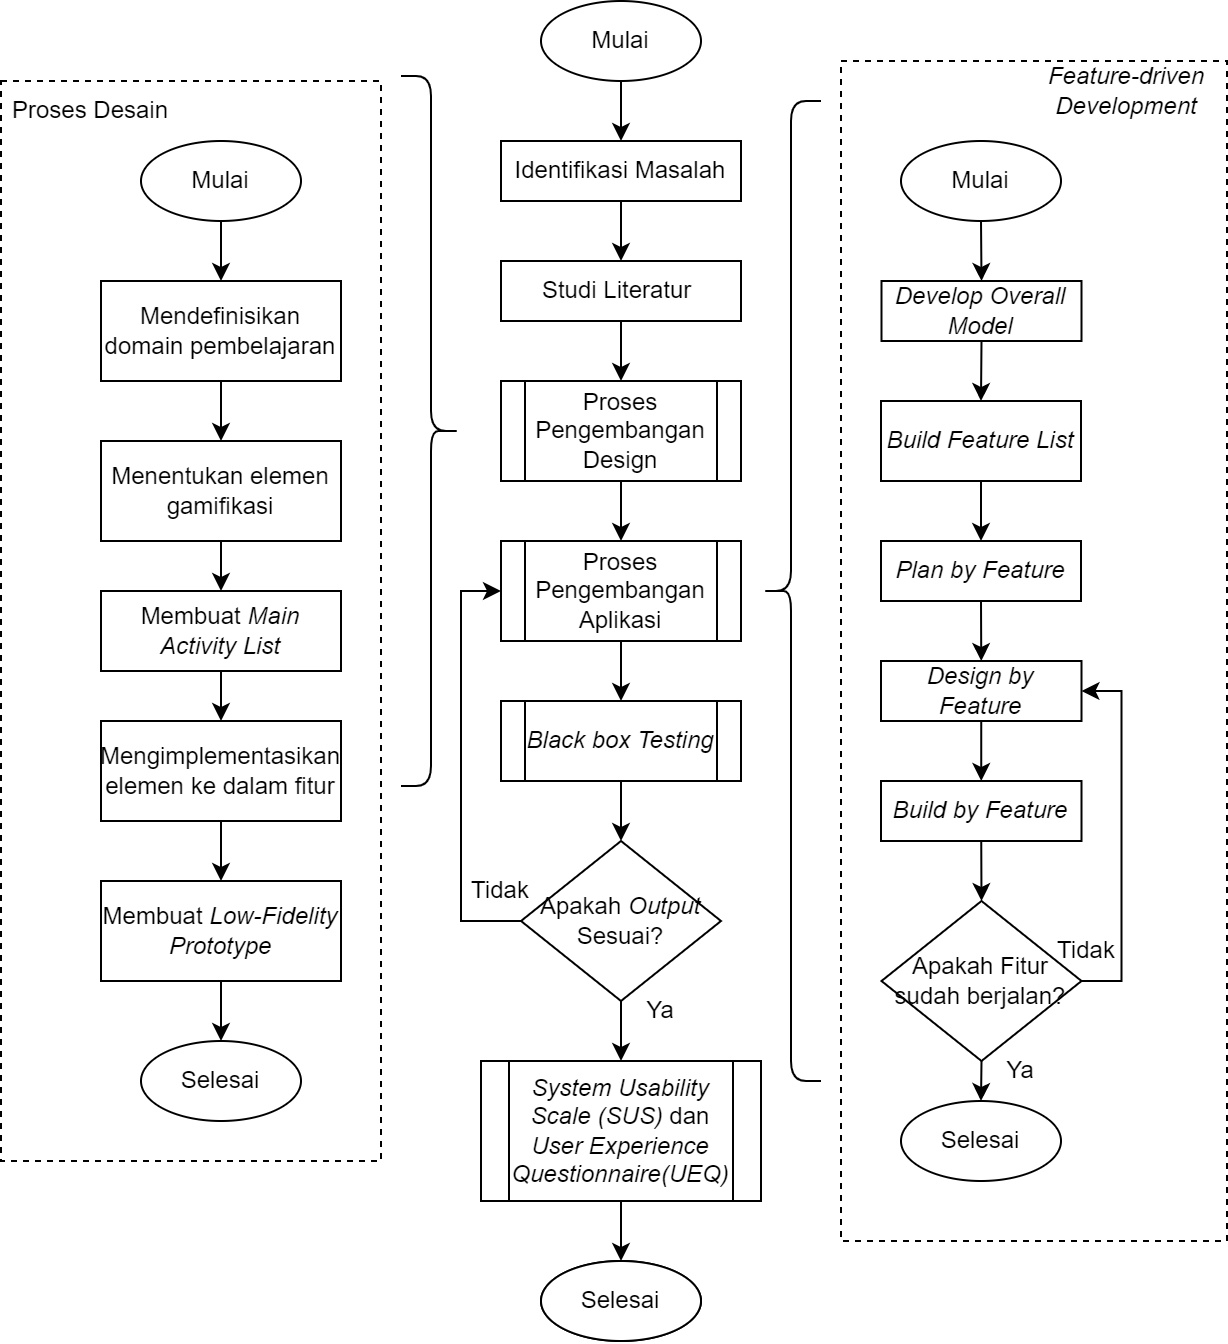
\includegraphics[width=12cm]{contents/chapter-3/images/Alur-tugas-akhir.png}
	\caption[Caption]{Alur Tugas Akhir}
	\label{Fig:Alur Tugas Akhir}
\end{figure}
% \section{Etika, Masalah, dan Keterbatasan Penelitian (Opsional)}
\subsection{Identifikasi Masalah}
\subsection{Studi Literatur}
\subsection{Observasi dan memperlajari Aplikasi dengan Gamifikasi}
\subsection{\textit{Develop Overall Model}}
\subsection{\textit{Build Feature List}}
% \subsection(\textit{Designing GAmification Based on Feature})
\subsection{\textit{Plan by Feature}}
\subsection{\textit{Design by Feature}}
\subsection{\textit{Build by Feature}}
\subsection{Menguji Fungsionalitas Aplikasi \textit{Black Box Testing}}
\subsection{Pengujian Aplikasi}

% Bagian ini membahas pertimbangan etis penelitian dan [potensi] masalah serta
% keterbatasannya. Jika menyangkut penelitian dengan makhluk hidup, maka dibutuhkan adanya \textit{ethical clearance}, di bagian ini hal itu akan dibahas. Demikian juga tentang keterbatasan ataupun masalah yang akan timbul.
